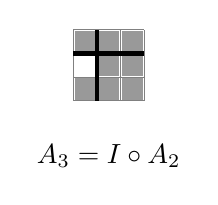
\begin{tikzpicture}
\draw[step=0.3cm,gray,thin] (0,0) grid (0.8999999999999999,0.8999999999999999);
\fill[black!40!white] (0.015,0.885) rectangle (0.285,0.6149999999999999);
\fill[black!40!white] (0.315,0.885) rectangle (0.585,0.6149999999999999);
\fill[black!40!white] (0.6149999999999999,0.885) rectangle (0.885,0.6149999999999999);
\fill[black!40!white] (0.315,0.585) rectangle (0.585,0.315);
\fill[black!40!white] (0.6149999999999999,0.585) rectangle (0.885,0.315);
\fill[black!40!white] (0.015,0.285) rectangle (0.285,0.015000000000000013);
\fill[black!40!white] (0.315,0.285) rectangle (0.585,0.015000000000000013);
\fill[black!40!white] (0.6149999999999999,0.285) rectangle (0.885,0.015000000000000013);
\draw[ultra thick] (0.3,0.0) -- (0.3,0.8999999999999999);
\draw[ultra thick] (0.0,0.6) -- (0.8999999999999999,0.6);
\node[] at (0.44999999999999996,-0.7) {  $A_{3}=I \circ A_2 $};\end{tikzpicture}